\providecommand{\main}{../..}
\documentclass[\main/main.tex]{subfiles}

%\graphicspath{ {\main/chapters/circuiti/}}

\begin{document}
\clearpage
\section{MOS equivalenti}
\subsection{MOS in serie}
\begin{figure}
	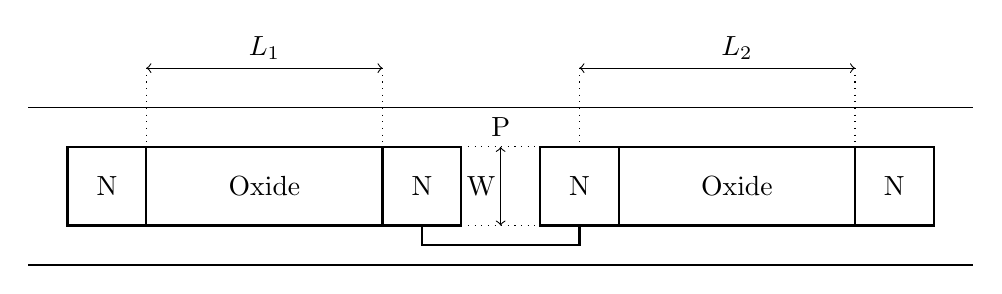
\begin{tikzpicture}[scale=0.5]
		%SEZIONE DAL ALTO

		% Silicon Top
		\draw (0,-4)  -- (24,-4);
		\draw (0,-8)  -- (24,-8);

		%Mos top
		\draw [fill=white, thick] (1,-5) rectangle (3,-7);
		\draw [fill=white, thick] (3,-5) rectangle (9,-7);
		\draw [fill=white, thick] (9,-5) rectangle (11,-7);

		%Mos top
		\draw [fill=white, thick] (13,-5) rectangle (15,-7);
		\draw [fill=white, thick] (15,-5) rectangle (21,-7);
		\draw [fill=white, thick] (21,-5) rectangle (23,-7);

		% Letters
		\node[] at (2,-6) {N};
		\node[] at (10,-6) {N};
		\node[] at (12,-4.5) {P};
		\node[] at (6,-6) {Oxide};

		% Letters
		\node[] at (14,-6) {N};
		\node[] at (22,-6) {N};
		\node[] at (18,-6) {Oxide};

		% L
		\draw [<->] (3,-3) -- (9,-3);
		\draw[dotted] (3,-3) -- (3,-5);
		\draw[dotted] (9,-3) -- (9,-5);
		\node[] at (6,-2.5) {$L_1$};

		% L
		\draw [<->] (14,-3) -- (21,-3);
		\draw[dotted] (14,-3) -- (14,-5);
		\draw[dotted] (21,-3) -- (21,-5);
		\node[] at (18,-2.5) {$L_2$};

		% W
		\draw [<->] (12,-7) -- (12,-5);
		\draw[dotted] (11,-7) -- (13,-7);
		\draw[dotted] (11,-5) -- (13,-5);
		\node[] at (11.5,-6) {W};

		\draw[thick] (10,-7) -- (10,-7.5) -- (14,-7.5) -- (14,-7);

	\end{tikzpicture}
	\caption{Vista in sezione e dal alto di due NMOS in serie}
\end{figure}

Due Mos in serie possono essere visti come un unico MOS con $L = L_1 + L_2$

E Poiche'
\[K_n =  \frac{1}{2} \mu_n C_{ox}'\left(\frac{W}{L}\right)\]
allora
\[K_{n,eq} =  \frac{1}{2} \mu_n C_{ox}'\left(\frac{W}{L_1+L_2}\right)\]

Quindi generalizzando avendo $n$ mos in serie
\[K_{n,eq} = \rnd{\sum_{i = 0}^{n} \frac{1}{K_i}}^{-1}\]
Quindi la SERIE tra MOS sostanzialmente e' uguale al PARALLELO tra resistenze.


\subsection{MOS in parallelo}
\begin{figure}
	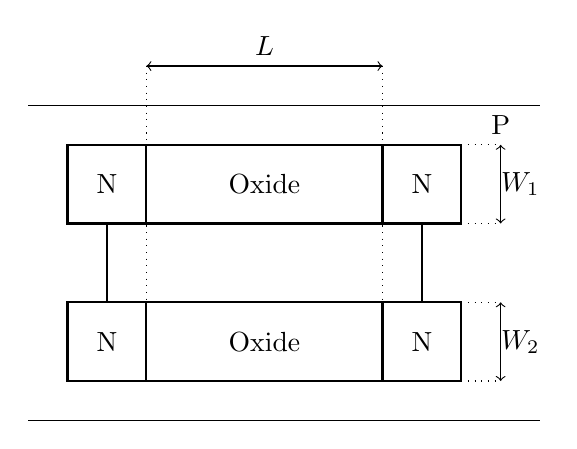
\begin{tikzpicture}[scale=0.5]
		%SEZIONE DAL ALTO

		% Silicon Top
		\draw (0,-4)  -- (13,-4);
		\draw (0,-12)  -- (13,-12);

		%Mos top
		\draw [fill=white, thick] (1,-5) rectangle (3,-7);
		\draw [fill=white, thick] (3,-5) rectangle (9,-7);
		\draw [fill=white, thick] (9,-5) rectangle (11,-7);
		%Mos top
		\draw [fill=white, thick] (1,-9) rectangle (3,-11);
		\draw [fill=white, thick] (3,-9) rectangle (9,-11);
		\draw [fill=white, thick] (9,-9) rectangle (11,-11);


		% Letters
		\node[] at (2,-6) {N};
		\node[] at (10,-6) {N};
		\node[] at (12,-4.5) {P};
		\node[] at (6,-6) {Oxide};

		% Letters
		\node[] at (2,-10) {N};
		\node[] at (10,-10) {N};
		\node[] at (6,-10) {Oxide};


		% L
		\draw [<->] (3,-3) -- (9,-3);
		\draw[dotted] (3,-3) -- (3,-9);
		\draw[dotted] (9,-3) -- (9,-9);
		\node[] at (6,-2.5) {$L$};


		% W
		\draw [<->] (12,-7) -- (12,-5);
		\draw[dotted] (11,-7) -- (12,-7);
		\draw[dotted] (11,-5) -- (12,-5);
		\node[] at (12.5,-6) {$W_1$};
		% W
		\draw [<->] (12,-11) -- (12,-9);
		\draw[dotted] (11,-11) -- (12,-11);
		\draw[dotted] (11,-9) -- (12,-9);
		\node[] at (12.5,-10) {$W_2$};

		\draw[thick] (2,-7) -- (2,-9);
		\draw[thick] (10,-7) -- (10,-9);


	\end{tikzpicture}
	\caption{Vista in sezione e dal alto di due NMOS in parallelo}
\end{figure}

Due Mos in serie possono essere visti come un unico MOS con $W = W_1 + W_2$

E Poiche'
\[K_n =  \frac{1}{2} \mu_n C_{ox}'\left(\frac{W}{L}\right)\]
allora
\[K_{n,eq} =  \frac{1}{2} \mu_n C_{ox}'\left(\frac{W_1 + W_2}{L}\right)\]

Quindi generalizzando avendo $n$ mos in serie
\[K_{n,eq} = \sum_{i = 0}^{n} K_i\]
Quindi il PARALLEO tra MOS sostanzialmente e' uguale alla SERIE tra resistenze.


\clearpage
\section{Porte Logiche}
Un importante utilizzo dei MOS e' per costruire porte logiche le quali sono usate in qualsiasi calcolatore e/o circuito digitale.

Vi sono vari modi per implementarle, ognuno con i suoi PRO e i suoi CONTRO, anche se lo standard al giorno d'oggi e' la logica CMOS.

L'idea e' di usare i MOS come interruttori per implementare la funzione logica $f(x_1,x_2,...,x_n)$.

E ovviamente poiche' uso i MOS come interruttori posso combinarli per creare reti che fanno combinazioni di AND ed OR degli ingressi.

I NOT li realizzo con porte a parte e/o con il tipo di Logica con cui sono Implementati

Per gli scopi logici possiamo approssimare il comportamento dei MOS alle seguenti tabelle di verita':

\begin{figure}
	\begin{subfigure}{.5\textwidth}
		\centering
		NMOS

		\begin{tabular}{ c | c }
			$V_G$ & Conduce? \\
			\hline
			"1"   & Si       \\
			"0"   & No       \\
		\end{tabular}
	\end{subfigure}%
	\begin{subfigure}{.5\textwidth}
		\centering
		PMOS

		\begin{tabular}{ c | c }
			$V_G$ & Conduce? \\
			\hline
			"1"   & No       \\
			"0"   & Si       \\
		\end{tabular}
	\end{subfigure}
\end{figure}


\subsection{Logica PullDown}

\begin{center}
	\begin{circuitikz}
		\draw (0,4) node[tground] {} (0,4)
		node[above] {$V_{dd}$} (0,4)
		to[resistor = R, i=$I_D$, -*] (0,1) ;
		\draw (0,1) to[short, -o] (2,1)  node[above] {$V_{out}$};
		\draw(0,1) to[generic] (0,-1) node[ground] {};
		\node[] at (1.5,0) {$f(x_1,x_2,...,x_n)$};
	\end{circuitikz}
\end{center}

Poiche' la rete e' tra massa e $V_{out}$ queste reti sono tipicamente implementate ad NMOS.

Quindi poiche' quando gli NMOS son spenti $V_{out} = "1"$ e quando sono accesi $V_{out} = "0"$ l'uscita e' negata rispetto alla funzione implementata.

Quindi $V_{out} = \neg f(x_1,x_2,...,x_n)$

Poi vi e' il problema del fatto che se $V_{out} = "0"$ vuol dire che i NMOS conducono quindi nel ramo vi sara' una corrente $I_{D}$ e quindi la tensione ai capi dei NMOS non sara' esattamente 0 ma $V_{dd} - R I_{D}$ che se la porta e' ben dimensionata puo' esser resa molto piccola.

Pero' rimane il fatto che se vi e' una corrente nel ramo allora vi e' consumo di potenza $P_{STAT} = V_{dd} I_{D} \neq 0W$ quindi la porta dissipa potenza per rimanere in questo stato.

\begin{center}
	\begin{tabular}{ c | c }
		PRO                 & CONTRO                    \\
		\hline
		Facile da costruire & "0" non effettivamente 0V \\
		Pochi componenti    & Potenza Statica $\neq 0W$ \\
	\end{tabular}
\end{center}

\clearpage
\subsection{Logica PullUp}
La logica PullUp e' duale alla PullDown quindi sono simili in molti aspetti.
\begin{center}
	\begin{circuitikz}
		\draw (0,4) node[tground] {} (0,4)
		node[above] {$V_{dd}$} (0,4)
		to[generic, i=$I_D$, -*] (0,1) ;
		\draw (0,1) to[short, -o] (2,1)  node[above] {$V_{out}$};
		\draw(0,1) to[resistor = R] (0,-1) node[ground] {};
		\node[] at (1.5,2.5) {$f(x_1,x_2,...,x_n)$};
	\end{circuitikz}
\end{center}

Poiche' tipicamente le reti di PullUp sono implementate coi PMOS il che le rende meno usate poiche' e' piu' difficile creare i PMOS che gli NMOS su un unico substrato.

I PMOS hanno tabella di verita' approssivamente:
\begin{center}
	\begin{tabular}{ c | c }
		$V_G$ & Conduce? \\
		\hline
		"1"   & No       \\
		"0"   & Si       \\
	\end{tabular}
\end{center}
quindi piu' realisticamente invece di $f(x_1,x_2,...,x_n)$ avro' una funzione del tipo $f(\neg x_1,\neg x_2,...,\neg x_n)$

quindi in questo caso vi e' corrente nel ramo quando $V_{out} = "1" = V_{dd}$ e quindi $V_{out}$ non e' esattamente $V_{dd}$ ma $V_{out} = R I_{D}$ che quindi non e' ideale e come precedentmente poiche' vi e' corrente vi e' dissipazione di energia per mantenere lo stato.

\begin{center}
	\begin{tabular}{ c | c }
		PRO                 & CONTRO                          \\
		\hline
		Facile da costruire & "1" non effettivamente $V_{dd}$ \\
		Pochi componenti    & Potenza Statica $\neq 0W$       \\
		Utilizza PMOS       &                                 \\
	\end{tabular}
\end{center}
\clearpage
\subsection{Logica CMOS}
La logica CMOS e' sostanzialmente l'unione della PullDown e della PullUp.

L'idea e' di avere Due reti cooperanti l'una il negato del altra.


\begin{center}
	\begin{circuitikz}
		\draw (0,4) node[tground] {} (0,4)
		node[above] {$V_{dd}$} (0,4)
		to[generic, i=$I_D$, -*] (0,1) ;
		\draw (0,1) to[short, -o] (2,1)  node[above] {$V_{out}$};
		\draw(0,1) to[generic] (0,-1) node[ground] {};
		\node[] at (1.5,2.5) {$\neg f(x_1,x_2,...,x_n)$};
		\node[] at (1.5,0) {$f(x_1,x_2,...,x_n)$};
	\end{circuitikz}
\end{center}

Si osserva che applicando il Teorema di De Morgan si puo' ottnere $\neg f_1(x_1,x_2,...,x_n) \rightarrow f_2(\neg x_1,\neg x_2,...,\neg x_n)$ a patto che si scambino $\wedge \longleftrightarrow \vee$ quindi Gli OR diventano AND e gli AND diventano OR.

Una buona caratteristica e' che poiche' ho due reti negate che cooperano sia con $V_{out} = "1"$ che con $V_{out} = "0"$ almeno una delle reti e' a "0" quindi non conduce, il che implica che, salvo i transitori di commutazione ,non vi sia passaggio di corrente.

Quindi non vi e' dissipazione di potenza e la rete che poiche' la corrente e' 0 i MOS anche se accesi avranno tensione $V_{SD} = 0V$ quindi i valori di $V_{out}$ sono esattamente $V_{dd}$ e $0V$

Quindi sostanzialmente si puo' implementare una rete di NMOS per la parte di PullDown e reinplementarla coi PMOS per la parte di PullUp semplicemente cambiando le serie con i paralleli e viceversa.

\begin{center}
	\begin{tabular}{ c | c }
		PRO                    & CONTRO                                \\
		\hline
		"0" ed "1" perfetti    & piu' difficili da costruire           \\
		Potenza Statica $= 0W$ & utilizzano PMOS                       \\
		                       & Piu' componenti delle altre soluzioni \\
	\end{tabular}
\end{center}

\clearpage
\end{document}